
% this file is called up by thesis.tex
% content in this file will be fed into the main document

%: ----------------------- introduction file header -----------------------
\begin{savequote}[50mm]
The logic of validation allows us to move between the two limits of dogmatism and skepticism. 
\qauthor{Paul Ricoeur}
\end{savequote}


\chapter{Evaluación}
\label{cha:Validation of the methodology}

% the code below specifies where the figures are stored
\ifpdf
    \graphicspath{{5_experiments_and_results/figures/PNG/}{5_experiments_and_results/figures/PDF/}{5_experiments_and_results/figures/}}
\else
    \graphicspath{{5_experiments_and_results/figures/EPS/}{5_experiments_and_results/figures/}}
\fi


%------------------------------------------------------------------------- 

En este capítulo se evalúa la idoneidad del método propuesto para la evaluación de competencias genéricas. Este capítulo se estructura de la siguiente manera:

\begin{itemize}
	\item En primer lugar se describen las características de los procedimientos que se han utilizado para llevar a cabo la evaluación:
		\begin{itemize}
			\item Publicaciones
			\item Cuestionarios
		\end{itemize}
	\item En segundo lugar se muestran los resultados de la aplicación en cada una de las actividades de aprendizaje para los que se ha implementado el método:
		\begin{itemize}
			\item Wikis: AMW
			\item VLE: SASQL Y EvalCourse
			\item Mundos virtuales: VWQL Y EvalSim
		\end{itemize}
	\item Finalmente se presentan las conclusiones de estas evaluaciones, tanto de los cuestionarios como de las publicaciones.
\end{itemize}

\section{Introducción}

La evaluación del método se ha realizado desde dos perspectivas. Por un lado, cada una de las implementaciones realizadas se ha tratado de mostrar tanto en congresos y revistas de relevancia en el área de las TEL. Mientras que por otro lado, se han realizado cuestionarios y entrevistas a profesionales de la enseñanza para evaluar la idoneidad de los indicadores obtenidos. A continuación se introducen ambos enfoques.

\subsection{Publicaciones}

Durante el desarrollo de este método se ha tratado de publicar en diferentes ámbitos a partir de cada una de sus implementaciones. La evaluación realizada en revistas de ímpacto y conferencias de relevancia son realizadas mediante procesos de \emph{revisión por par doble-ciego}, donde tanto los revisores como los autores son anónimos~\cite{ladron2008revision}. De esta forma se han recibido evaluaciones, opiniones y recomendaciones, que se han ido incorporando a las diferentes implementaciones y al método.

\subsection{Cuestionarios y entrevistas}

En el transcurso de esta tesis se ha presentado en varios foros el trabajo que se va desarrollando. Los profesionales de la educación que han asistido a las presentaciones han participado en cuestionarios de evaluación de la propuesta y han vertido sus opiniones y recomendaciones sobre el método en las entrevistas realizadas. Los profesionales que han participado son profesores universitarios, profesores de primaria y secundaria y personal de MediaWiki España.

\section{AMW aplicado a MediaWiki}

Integer fermentum rutrum urna at vestibulum. Vivamus ullamcorper erat in sapien dignissim pellentesque. Integer convallis fringilla dictum. In bibendum lectus eu nulla pretium volutpat. Morbi hendrerit fringilla tortor, sed gravida neque lacinia a. In risus magna, hendrerit vitae cursus ac, vehicula at eros. Aenean quis ipsum sit amet leo vestibulum cursus.

\section{EvalCourse aplicado a entornos de apredizaje virtual}

Los estudios de caso que se presentan en este capítulo fueron publicados en la revista~\emph{International Journal of Engineering Education, Special issue on Innovative Methods of Teaching Engineering}~\cite{Balderas:2015}, después de haber sido invitados a extender un primer trabajo presentado en el~\emph{4th International Workshop on Software Engineering for E-learning (ISELEAR’13)}~\cite{balderas2013generative}.

\subsection{Evaluación}

Los estudios de caso en los que se aplicó EvalCourse tuvieron lugar en dos asignaturas de la titulación de Ingenieria Informática de la Universidad de Cádiz, en el curso 2012/13. La evaluación del curso se realizó de forma manual, y después se aplicó EvalCourse para evaluar a los estudiantes en las competencias de liderazgo, habilidades interpersonales y autocrítica.

\subsubsection{Extracción de indicadores del foro}

El primero de los casos de estudio tuvo lugar en la asignatura de \emph{Procesadores de Lenguajes II} y que tenía 36 estudiantes matriculados. Era una asignatura obligatoria, que tenía lugar en el primer semestre del quinto (y último) curso. Durante el semestre, los estudiantes tuvieron que trabajar en pequeños equipos de dos o tres miembros. Cada equipo del curso tenía un foro para la comunicación interna. Este foro se utilizó para evaluar dos competencias: habilidades interpersonales y liderazgo.

En primer lugar, como indicador de las habilidades interpersonales de cada estudiante se calculó el total de intervenciones en el foro. El coordinador del curso animó a sus estudiantes a participar en el foro del equipo, ya que debía ser su herramienta de comunicación interna. Un estudiante que tenía tres o más intervenciones en el foro tendría una buena calificación. En segundo lugar, como indicador de liderazgo se consideró los debates que los estudiantes iniciaron en el foro. Un estudiante que inició dos o más debates tuvo una calificación positiva en la competencia de liderazgo.

\paragraph*{Análisis}

Sólo 18 de los 36 estudiantes del curso participaron en los foros. No se puede determinar que los estudiantes que no participaron en el foro no posean las competencias, lo único que podemos afirmar es que no demostraron su desempeño en estas competencias a través de esta actividad. Los resultados de haber aplicado EvalCourse pueden verse en el listado de la tabla~\ref{tab:EvcEvaluacionListadoForo1}. Pocos estudiantes obtuvieron una calificación positiva en estas competencias, habiendo varios estudiantes que destacan sobre el resto. Estos datos se exportaron a una hoja de cálculo y se genero la figura~\ref{fig:EvcEvaluacionTartaForo1}. En resumen, consideramos que los estudiantes, a pesar de que sabían que debían utilizar el foro para la comunicación entre los miembros del equipo, no lo hicieron en su mayoría.

\begin{table}
	\centering
	\caption{Listado de intervenciones de los estudiante en el foro.}
	\label{tab:EvcEvaluacionListadoForo1}
	\begin{tabular}{|c|l|c|c|c|}
		\hline
		id & username & Debate- & Debate- & Total  \\
			&		&	starter	& participation		&		\\
		\hline
		\hline
		43 &	S2 &	0 &	1 &	 1 \\
		44 &	S3 &	3 &	4 &	 7 \\
		45 &	S4 &	2 &	2 &	 4 \\
		46 &	S5 &	0 &	1 &	 1 \\
		48 &	S7 &	4 &	3 &	 7 \\
		50 &	S9 &	6 &	8 &	 14 \\
		51 &	S10 &	1 &	1 &	 2 \\
		53 &	S12 &	0 &	1 &	 1 \\
		55 &	S14 &	1 &	1 &	 2 \\
		59 &	S18 &	1 &	2 &	 3 \\
		60 &	S19 &	2 &	0 &	 2 \\
		61 &	S20 &	0 &	2 &	 2 \\
		62 &	S21 &	0 &	1 &	 1 \\
		67 &	S26 &	0 &	1 &	 1 \\
		70 &	S29 &	0 &	1 &	 1 \\
		71 &	S30 &	2 &	1 &	 3 \\
		75 &	S34 &	1 &	5 &	 6 \\
		78 &	S37 &	2 &	4 &	 6 \\
		\hline
	\end{tabular}
\end{table}

\begin{figure}
	\centering
	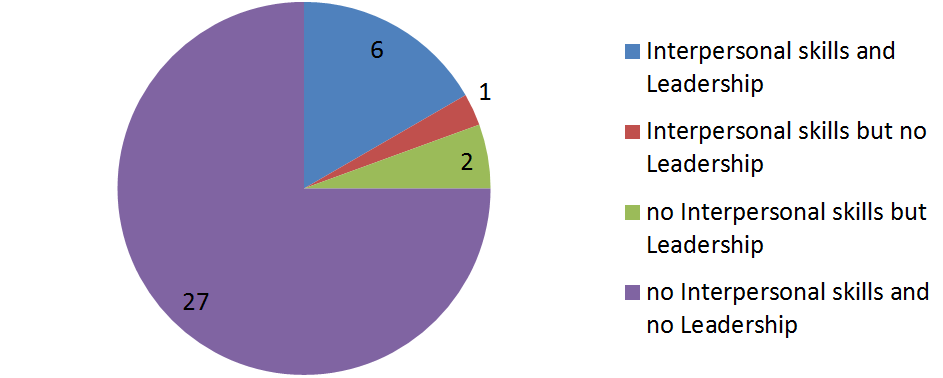
\includegraphics[width=12cm]{EvcForo1.png}
	\caption{Resumen del desempeño de los estudiantes en el foro en las dos competencias.}
	\label{fig:EvcEvaluacionTartaForo1}
\end{figure}

A pesar de esto, de manera informal sí se observó que los estudiantes con calificaciones positivas en ambas competencias realmente tuvieron un buen desempeño de dichas competencias en la asignatura. Por tanto, pudimos decir que los indicadores elegidos parecían ser verdaderas evidencias del nivel de competencia de los estudiantes. Probablemente el hecho de que el varlos dado a la participación en el foro en la calificación global de la asignatura fuera sólo de un 2,5\percentage no animó a los estudiantes a no utilizar en exclusiva sus habituales métodos de comunicación (Whatsapp, correo electronico, reuniones en el pasillo, etc.).

También se utilizó EvalCourse para analizar la interacción entre los estudiantes. La idea era localizar interacciones que quizás estuviese más interesadas en mejorar sus resultados que en la mera comunicación. Se detectaron evidencias de interacciones fraudulentas entre dos estudiantes cuando se podía ver que ellos sólo estaban interesados en hablar entre ellos dos y no habían interactuado con ningún otro compañero. Con el código SASQL mostrado en la consulta~\ref{code:interaction1} se obtuvo la interacción que hubo en el foro. Los resultados se pueden ver en la figura~\ref{fig:EvcEvaluacionInteraccionForo2}.


\begin{lstlisting}[caption=Código SASQL para extraer datos sobre la interacción en el foro ,label=code:interaction1,numbers=left, captionpos=b, morekeywords={Evidence,get, students, show, milestones, participation, access, in, assignment, forum, campus, workshop, interaction}]
Evidence forum_interaction: 
	get students
	show interaction
	in forum.
\end{lstlisting}

\begin{figure}
	\centering
	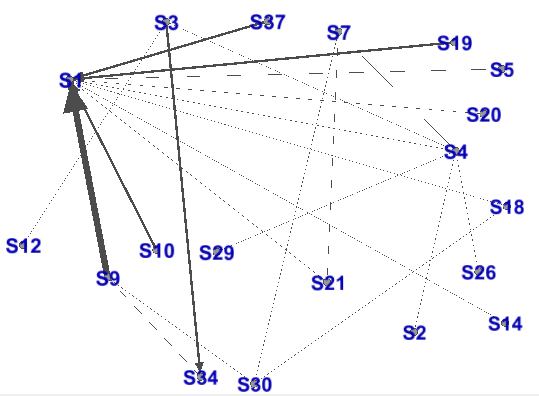
\includegraphics[width=12cm]{EvcForo2.png}
	\caption{Graph of students' interaction in forum case study.}
	\label{fig:EvcEvaluacionInteraccionForo2}
\end{figure}

Concluímos que gran parte de la interacción del foro se debía a mensajes de respuesta al profesor (S1). Esto hecho es un indicio de que en muchos casos la interacción de los estudiantes con el foro es más debida a cuestiones que los estudiantes realizan al profesor para que les aclaren algunas de las intrucciones proporcionadas en el propio foro que al uso del foro como herramienta del grupo.

\subsubsection{Extracción de indicadores del taller}

El segundo estudio de caso que se analizó se desarrolló en la asignatura de Programación Funcional, en la que había 19 estudiantes matriculados. Esta es una asignatura optativa que tiene lugar también en el segundo semestre del quinto (y último) curso. Los estudiantes tuvieron que trabajar en cuatro talleres a lo largo del curso. En Moodle, un taller es un entregable que, conforme a las intrucciones del profesor, puede ser evaluado por otro u otros estudiantes o auto-evaluado. Los estudiantes debían entregar una tarea en un taller habilitado para cada tema antes de la fecha límite fijada en la actividad. Tras la fecha de entrega, el profesor proporcionaba la solución a la tarea, de manera que cada tarea fuera evaluada por dos compañeros de manera aleatoria y por el propio estudiante. A final de curso, se calculó la media de las calificaciones de todos los talleres. Esta calificación era el 30\percentage de la nota de la asignatura, siendo obligatoria una buena calificación para aprobar la asignatura. El profesor de la asignatura tenía que evaluar la capacidad de autocrítica de sus estudiantes. Para ello, utilizó como indicador para cada tarea la diferencia entre la media de las calificaciones dadas por cada compañero con respecto a la calificación que se asignó el propio estudiante. Cada estudiante evaluaba su propio trabajo antes de saber la calificación que le habían dado sus compañeros.

El grado de validez del indicador proporcionado por EvalCourse dependerá del profesor, que si lo considera oportuno, podrá contrastar o complementar el indicador con otros actividades de aprendizaje. Al igual que los estudiantes deben haber sido instruídos para realizar el trabajo que se les pedia, deben ser capaces de evaluar el trabajo de sus compañeros, argumentando sus criterios, sus razones y sus evidencias.

\paragraph*{Análisis}

A partir del código mostrado en la consulta~\ref{code:EvcWorkshop1}, se obtiene el listado~\ref{tab:EvcWorkshop1} con los indicadores que se utilizaron para evaluar a los estudiantes en la competencia de la autocrítica (en un rango de 0 a 10). En la figura~\ref{fig:EvcWorkshop1} se muestra un grafo con la diferencia entre sus auto-calificaciones y las otorgadas por sus compañeros. Este grafo se genero a partir de la iimportación de los indicadores a una hoja de cálculo. En él, se detecta fácilmente a dos estudiantes que se auto-asignaron una calificación inferior a la que le dieron sus compañeros.

\begin{lstlisting}[caption=Extracción evaluaciones realizadas en los talleres ,label=code:EvcWorkshop1,numbers=left, captionpos=b, morekeywords={Evidence,get, students, show, milestones, evaluations, participation, access, in, assignment, forum, campus, between, and, workshop, interaction}]
Evidence workshop_critical: 
	get students
	show evaluations
	in workshop.
\end{lstlisting}

\begin{table}
	\centering
	\caption{Desempeño de los estudiantes en la competencia de la autocrítca.}
	\label{tab:EvcWorkshop1}
	\begin{tabular}{|l|c|c|c|}
		\hline
		username & Peer-grade & Self-grade & Mean-diff \\
		\hline
		\hline
			Stud3 & 5.26 & 5.56 & 0.3 \\
			Stud6 & 6.22 & 7.06 & 0.94 \\
			Stud7 & 5.92 & 7.44 & 1.52 \\
			Stud8 & 7.62 & 8.03 & 0.60 \\
			Stud9 & 9.38 & 9.33 & 0.57 \\
			Stud10 & 7.39 & 8.14 & 0.75 \\
			Stud11 & 5.24 & 5.64 & 0.62 \\
			Stud12 & 7.30 & 6.80 & 0.83 \\
			Stud13 & 8.06 & 7.92 & 0.55 \\
			Stud14 & 9.92 & 9.86 & 0.22 \\
			Stud15 & 5.12 & 6.00 & 1.43 \\
			Stud16 & 7.85 & 7.06 & 0.79 \\
			Stud17 & 9.00 & 8.97 & 0.75 \\
			Stud18 & 6.29 & 7.31 & 1.01 \\
			Stud22 & 7.16 & 8.20 & 1.03 \\
			Stud25 & 8.61 & 8.72 & 0.22 \\
			Stud28 & 8.14 & 8.08 & 0.47 \\
			Stud30 & 9.54 & 9.44 & 0.23 \\
		\hline
	\end{tabular}
\end{table}

\begin{figure}
	\centering
	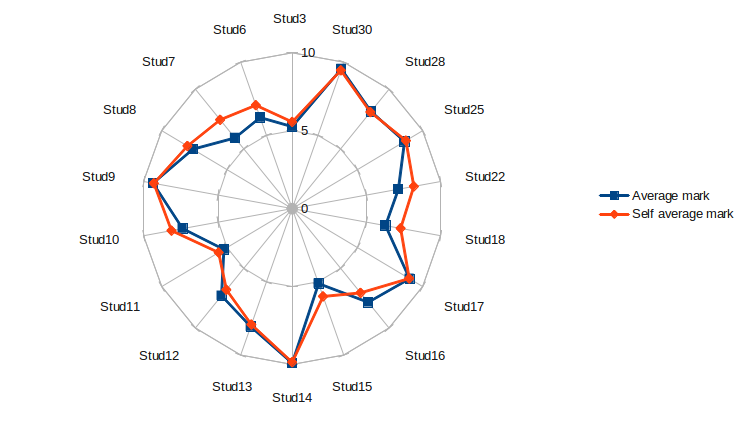
\includegraphics[width=12cm]{EvcWorkshop1.png}
	\caption{Grafo que muestra las diferentes calificaciones que se autoasignaron los estudiantes y la que les dieron sus compañeros.}
	\label{fig:EvcWorkshop1}
\end{figure}

Se puede decir que no hubo muchas diferencias en las calificaciones. Esto es un buen indicador, ya que la mayor parte de los estudiantes que tuvieron una diferencia grande en las primeras calificaciones, corrigieron esta desviación en las siguientes evaluaciones. Aunque también hay estudiantes que hicieron buenas auto-evaluaciones desde el principio, como se puede comprobar viendo la última columna de la tabla~\ref{tab:EvcWorkshop1}. En ella se representa la diferencia media de las calificaciones que recibieron y que se autoasignaron.

En este punto el profesor tuvo que decidir sobre la validez del indicador. Y en caso afirmativo, cuál seria el límite entre una valoración positiva y una negativa. Gracias a que el grupo era pequeño, el profesor podía comparar el comportamiento real observado durante el curso con los resultados del indicador, confirmando que había mucha similitud entre ambas calificaicones. De hecho, el límite positivo se estableció con una media de $0,5$ puntos o menos. Mientras que una valoración negativa se dejó para aquellos cuya diferencia era superior a $1$. Con estos resultados se obtuvo la siguiente distribución (provocando una distribución de campana).

\begin{itemize}
\item Si la diferencia media está entre $0$ y $0,5$, esto era un indicador positivo del desempeño de la competencia de la autocritica. (5 estudiantes).
\item Si la diferencia media está entre $0,5$ y $1$, los estudiantes mostraron un nivel medio de la competencia (9 estudiantes).
\item If the mean difference of the averages is $1$ or higher, esto era un indicador negativo del desempeño de la competencia de la autocritica (4 estudiantes).
\end{itemize}

Por supuesto, se necesitan más estudios para determinar la validez de los resultados de EvalCourse como indicadores de la competencia. Sin embargo, en nuestro caso, pudimos decir que la informaicón fue de utilidad para justificar la evaluación de los estudiantes.

\subsection{Resultados}

Morbi at augue sapien. Duis tempus quam vitae velit interdum ultricies. Vivamus laoreet lacinia elit sit amet vehicula. Ut congue diam ac magna hendrerit sed fermentum justo lacinia. Curabitur vel odio neque, quis consequat mi. Proin lobortis justo quis enim fermentum accumsan sagittis ipsum imperdiet. Proin sem felis, laoreet placerat egestas id, fringilla id mauris. Pellentesque a nisi sit amet leo consectetur gravida nec et dui. Curabitur quis hendrerit augue. Etiam sed dui nec tortor convallis fringilla. Proin tempor mattis diam nec egestas. Quisque condimentum elementum lacus ac porta.

\section{EvalSim aplicado a los mundos virtuales}

Morbi at augue sapien. Duis tempus quam vitae velit interdum ultricies. Vivamus laoreet lacinia elit sit amet vehicula. Ut congue diam ac magna hendrerit sed fermentum justo lacinia. Curabitur vel odio neque, quis consequat mi. Proin lobortis justo quis enim fermentum accumsan sagittis ipsum imperdiet. Proin sem felis, laoreet placerat egestas id, fringilla id mauris. Pellentesque a nisi sit amet leo consectetur gravida nec et dui. Curabitur quis hendrerit augue. Etiam sed dui nec tortor convallis fringilla. Proin tempor mattis diam nec egestas. Quisque condimentum elementum lacus ac porta. Vivamus congue, odio eu ullamcorper elementum, leo turpis tempus sem, at condimentum dolor quam eu nunc. Pellentesque eget risus ac velit aliquam sollicitudin sed et ipsum. 

\section{Evaluación}

Morbi at augue sapien. Duis tempus quam vitae velit interdum ultricies. Vivamus laoreet lacinia elit sit amet vehicula. Ut congue diam ac magna hendrerit sed fermentum justo lacinia. Curabitur vel odio neque, quis consequat mi. Proin lobortis justo quis enim fermentum accumsan sagittis ipsum imperdiet. Proin sem felis, laoreet placerat egestas id, fringilla id mauris. Pellentesque a nisi sit amet leo consectetur gravida nec et dui. Curabitur quis hendrerit augue. Etiam sed dui nec tortor convallis fringilla. Proin tempor mattis diam nec egestas. Quisque condimentum elementum lacus ac porta. Vivamus congue, odio eu ullamcorper elementum, leo turpis tempus sem, at condimentum dolor quam eu nunc. Pellentesque eget risus ac velit aliquam sollicitudin sed et ipsum. 

\section{Conclusiones}

Morbi at augue sapien. Duis tempus quam vitae velit interdum ultricies. Vivamus laoreet lacinia elit sit amet vehicula. Ut congue diam ac magna hendrerit sed fermentum justo lacinia. Curabitur vel odio neque, quis consequat mi. Proin lobortis justo quis enim fermentum accumsan sagittis ipsum imperdiet. Proin sem felis, laoreet placerat egestas id, fringilla id mauris. Pellentesque a nisi sit amet leo consectetur gravida nec et dui. Curabitur quis hendrerit augue. Etiam sed dui nec tortor convallis fringilla. Proin tempor mattis diam nec egestas. Quisque condimentum elementum lacus ac porta. Vivamus congue, odio eu ullamcorper elementum, leo turpis tempus sem, at condimentum dolor quam eu nunc. Pellentesque eget risus ac velit aliquam sollicitudin sed et ipsum. 








% ----------------------------------------------------------------------

